% Theory part of the module.
%
% Module TH-9 of Section 6.7 of the syllabus: "The machine learning
% paradigm. Rules that a programmer writes and rules that a model learns
% from data. Features, labels, model, and loss. Regression and
% classification. Training and inference." Type T, 50 minutes.
%
% Sources: the slide decks and the reading of the HarvardX TinyML
% courseware (2-1-1 the two paradigms, 2-1-3 the loss, 2-2-6 from regression
% to classification, reading 2-1-10 the parameters of a neuron), and Volume I
% chapter 5 of the textbook (the rule-based limits, the feature
% engineering step, the automatic pattern discovery, the training loop, and
% the inference pipeline). The syllabus also names chapter 4.1 of XIAO: Big
% Power, Small Board, but no frame of this module uses it, so the credits
% frame does not name that book. The exercise is the one of the syllabus:
% decide if three problems need written rules or a learned model.
%
% The numbers of this module have three origins. Each frame says so in its
% source line.
% 1. A number that a source reports: the run of the courseware on six
%    points, the counts of MNIST, and the arithmetic of the running
%    example of Volume I, chapter 5.
% 2. The illustrative cost model of the chapter. Nobody measured it on a
%    board. The source line says so.
% 3. A value of this course: none. The module uses no measurement of the
%    course.
%
% Size: 15 to 25 frames for 50 minutes of theory.
%
% Three figures are adopted from the sources. The other diagrams are drawn
% again with TikZ. Rule 3 of ATTRIBUTION.md gives the source of each
% adopted figure and the change of each redrawn diagram.

% ------------------------------------------------- 1. the same task, two ways
\begin{frame}{The same task, two ways}
  \small A device must tell three movements apart: waving, flipping, and
  idling. One team writes the program. Another team records the movements
  and lets a program find the pattern.
  \vskip 0.4em
  \begin{itemize}
    \item Both teams end with a program that runs on the device.
    \item The rules live in a different place. In the first team a
          programmer wrote every rule. In the second team the data holds
          the rules.
  \end{itemize}
  \vskip 0.4em
  \keypoint{The question is not whether to use machine learning. The
  question is who writes the rules.}
\end{frame}

% --------------------------------------------- 2. the traditional paradigm
\begin{frame}{Written rules and data give answers}
  \begingroup\centering
  \begin{tikzpicture}[font=\scriptsize, >=stealth,
      bx/.style={draw=coolgray, rounded corners=2pt, fill=boxgray,
                 align=center, text width=2.2cm, minimum height=0.7cm},
      mid/.style={draw=cardinalred, rounded corners=2pt, fill=cardinalred!12,
                  align=center, text width=2.8cm, minimum height=0.9cm,
                  font=\scriptsize\sffamily\bfseries}]
    \node[bx] (r) at (0,0.85)  {Rules};
    \node[bx] (d) at (0,-0.85) {Data};
    \node[mid] (p) at (3.9,0)   {The program};
    \node[bx] (a) at (7.8,0)   {Answers};
    \draw[->] (r.east) -- (p.west);
    \draw[->] (d.east) -- (p.west);
    \draw[->] (p.east) -- (a.west);
  \end{tikzpicture}\par\endgroup
  \vskip 0.6em
  \small The programmer writes the rules first. The data arrives later, and
  the program applies the rules to it.
  \vskip 0.3em
  \keypoint{The rules are an input of the program.}
\end{frame}

% ------------------------------------------------ 3. where written rules hold
\begin{frame}{Where written rules hold}
  \small A game needs a rule for a collision, because the physics of the
  game is known and it never changes.
  \vskip 0.4em
  \begin{itemize}
    \item The states are few, and a person can list all of them.
    \item The correct answer is exact. No answer is close enough.
    \item A wrong answer is visible at once. The game looks broken.
  \end{itemize}
  \vskip 0.4em
  \small A thermostat with a fixed threshold is the same case: the rule is
  one line, and its test is a measurement of a number.
\end{frame}

% ------------------------------------------------ 4. where written rules break
\begin{frame}{Where written rules break}
  \begingroup\centering
  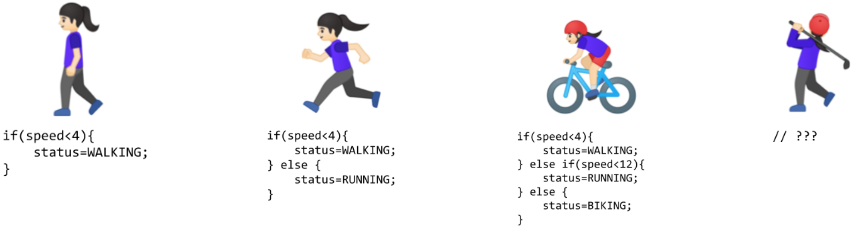
\includegraphics[width=0.86\textwidth]{images/modules/TH-9/activity_rules.png}
  \par\endgroup
  \vskip 0.4em
  \small The rule for walking is one test. Biking needs a second test. A
  movement that nobody wrote down needs a new branch, and no end is in
  sight.
  \source{Figure adopted from Volume I, chapter 5.}
\end{frame}

% --------------------------------------------------- 5. the cost of one more
\begin{frame}{The cost of one more rule}
  \footnotesize
  \begin{tabular}{@{}L{3.6cm}L{2.4cm}L{2.6cm}@{}}
    \toprule
    Movements named & Branches in the code & Lines to maintain \\
    \midrule
    2 & 2 & about 10 \\
    3 & 3 & about 15 \\
    4 & 4 & about 20 \\
    \bottomrule
  \end{tabular}
  \vskip 0.5em
  \small The count of branches follows the count of movements, and the
  count of movements follows the people who use the device. The code is
  correct at every step and wrong at the end, because the last movement is
  missing.
  \source{Illustration of this course, after the growth of the rule count in
    Volume I, chapter 5. Nobody measured these line counts.}
\end{frame}

% ------------------------------------------------ 6. the machine learning box
\begin{frame}{Data and answers give rules}
  \begingroup\centering
  \begin{tikzpicture}[font=\scriptsize, >=stealth,
      bx/.style={draw=coolgray, rounded corners=2pt, fill=boxgray,
                 align=center, text width=2.2cm, minimum height=0.7cm},
      mid/.style={draw=cardinalred, rounded corners=2pt, fill=cardinalred!12,
                  align=center, text width=2.8cm, minimum height=0.9cm,
                  font=\scriptsize\sffamily\bfseries}]
    \node[bx] (d) at (0,0.85)  {Data};
    \node[bx] (l) at (0,-0.85) {Answers};
    \node[mid] (m) at (3.9,0)   {The model};
    \node[bx] (r) at (7.8,0)   {Rules};
    \draw[->] (d.east) -- (m.west);
    \draw[->] (l.east) -- (m.west);
    \draw[->] (m.east) -- (r.west);
  \end{tikzpicture}\par\endgroup
  \vskip 0.6em
  \small The program no longer holds the rules. It finds them, and it holds
  the result.
  \vskip 0.3em
  \keypoint{The rules are the output of the program.}
\end{frame}

% ------------------------------------------------------- 7. what a model is
\begin{frame}{What a model is}
  \begin{equation*}
    \text{answer} = f(\text{input};\, \theta)
  \end{equation*}
  \small
  \begin{itemize}
    \item $f$ is the shape of the computation. It never changes after the
          training.
    \item $\theta$ holds the parameters: the weights and the biases. The
          training moves them.
    \item A neuron of the simplest kind has two parameters. Its output is
          \code{weight * input + bias}, so for the six points of the next
          frames the weight becomes 2 and the bias becomes $-1$.
  \end{itemize}
\end{frame}

% --------------------------------------------------------- 8. the four parts
\begin{frame}{The four parts of a learned model}
  \footnotesize
  \begin{tabular}{@{}L{2.4cm}L{4.1cm}L{3.0cm}@{}}
    \toprule
    Part & What it is & Who gives it \\
    \midrule
    Features & The input as a vector of numbers & The sensors, the code \\
    Labels & The right answer for each example & A person, most of the time \\
    Model & The function $f$ and its parameters $\theta$ & The training \\
    Loss & One number for the distance to the labels & The choice of the team \\
    \bottomrule
  \end{tabular}
  \vskip 0.5em
  \small Three of the four parts come from the team. The fourth is what the
  training produces.
\end{frame}

% -------------------------------------------------------------- 9. features
\begin{frame}{Features}
  \small A feature is a number that describes one thing about the input.
  \vskip 0.3em
  \begin{itemize}
    \item An accelerometer of a waving hand gives three numbers at each
          sample: the acceleration on the three axes. The sample rate adds
          the time.
    \item A photograph is already a vector of numbers: 784 grey values for
          a 28 by 28 image.
    \item The engineer chooses the features. A feature that the sensor does
          not measure needs another sensor or another code.
  \end{itemize}
  \vskip 0.3em
  \small The features of the classic example are the 784 pixel values of one
  handwritten digit.
  \source{Dimensions of the running example of Volume I, chapter 5.}
\end{frame}

% --------------------------------------------------------------- 10. labels
\begin{frame}{Labels}
  \small A label is the answer that belongs to one example.
  \vskip 0.3em
  \begin{itemize}
    \item For the six points of the regression, the label of each $x$ is
          its $y$.
    \item For a movement, the label is the name of the movement.
    \item The label of a digit is its number.
    \item Getting the labels is the slow part of the work. A radiologist
          reads each image, and two readers disagree on the border cases.
  \end{itemize}
  \vskip 0.3em
  \keypoint{The model is only as good as the labels.}
\end{frame}

% ------------------------------------------------------------- 11. the loss
\begin{frame}{The loss measures one number}
  \small Take six points. The real values are
  $y = \{-3, -1, 1, 3, 5, 7\}$ and a guess is $\hat{y} = 3x - 1$.
  \vskip 0.3em
  \footnotesize
  \begin{tabular}{@{}lrrrrrr@{}}
    \toprule
    $x$   & $-1$ & $0$ & $1$ & $2$ & $3$ & $4$ \\
    $\hat{y}$ & $-4$ & $-1$ & $2$ & $5$ & $8$ & $11$ \\
    $\hat{y} - y$ & $-1$ & $0$ & $1$ & $2$ & $3$ & $4$ \\
    \bottomrule
  \end{tabular}
  \vskip 0.5em
  \small The training needs one number, not six. The root mean square of
  the six differences is $\sqrt{31} = 5.57$.
\end{frame}

% ------------------------------------------------ 12. the loss guides the step
\begin{frame}{The loss guides every step of the training}
  \small The training does two things again and again: it predicts, then it
  measures.
  \vskip 0.3em
  \begin{itemize}
    \item A guess with a loss of 5.57 is worse than a guess with a loss of
          0.5. The number gives the order.
    \item The training moves the parameters in the direction that lowers
          the loss.
    \item A guess that fits the six points exactly, $y = 2x - 1$, has a
          loss of 0.
  \end{itemize}
  \vskip 0.3em
  \small \textbf{Loss:} one number for the distance between the answers of
  the model and the labels.
\end{frame}

% ------------------------------------------------------- 13. the train loop
\begin{frame}{Training is a loop}
  \begingroup\centering
  \begin{tikzpicture}[font=\scriptsize, >=stealth,
      bx/.style={draw=coolgray, rounded corners=2pt, fill=boxgray,
                 align=center, text width=2.15cm, minimum height=0.75cm}]
    \node[bx] (f) at (0,0)    {Predict\\ with the current $\theta$};
    \node[bx] (l) at (2.6,0)  {Measure\\ the loss};
    \node[bx] (g) at (5.2,0)  {Compute\\ the change};
    \node[bx] (u) at (7.8,0)  {Move $\theta$\\ a little};
    \draw[->] (f) -- (l); \draw[->] (l) -- (g); \draw[->] (g) -- (u);
    \draw[->, cardinalred, dashed] (u.south) -- ++(0,-1.0)
      -| node[pos=0.5, below, font=\scriptsize, text=cardinalred]
      {again, until the loss stops falling} (f.south);
  \end{tikzpicture}\par\endgroup
  \vskip 0.6em
  \small A network starts with random parameters, so its first prediction is
  close to a guess of ten classes with no information. Each turn of the
  loop makes the next prediction a little better.
\end{frame}

% --------------------------------------------------------- 14. what training is
\begin{frame}{What training is, in one line}
  \small
  \begin{quote}
    Show the model examples with their labels, and move the parameters so
    that the loss falls.
  \end{quote}
  \vskip 0.3em
  \begin{itemize}
    \item The examples come from a dataset. The dataset of the classic
          example holds 60 000 training images and 10 000 validation
          images.
    \item The moves are small. A step that is too large passes over the
          answer and the loss rises again.
    \item The loop ends when the loss on unseen examples stops falling.
  \end{itemize}
\end{frame}

% ------------------------------------------------------------ 15. inference
\begin{frame}{Inference is the forward pass alone}
  \begingroup\centering
  \begin{tikzpicture}[font=\scriptsize, >=stealth,
      bx/.style={draw=coolgray, rounded corners=2pt, fill=boxgray,
                 align=center, text width=2.3cm, minimum height=0.75cm}]
    \node[bx] (x) at (0,0)  {Input};
    \node[bx] (y) at (3.4,0){Prediction};
    \draw[->, thick] (x) -- (y);
    \node[font=\scriptsize, text=coolgray] at (1.7,0.62) {with frozen $\theta$};
    \draw[->, cardinalred, dashed] (y.south) -- ++(0,-1.75);
    \node[font=\scriptsize, text=cardinalred, align=center, fill=white,
          inner sep=1.5pt] at (3.4,-1.05) {no gradients,\\no labels};
  \end{tikzpicture}\par\endgroup
  \vskip 0.6em
  \small Inference runs the forward pass and stops. It keeps no gradients
  and no labels, so it needs far less memory than the training.
  \vskip 0.3em
  \keypoint{The training needs a big machine. The inference runs on the
  device.}
\end{frame}

% -------------------------------------------------- 16. training vs inference
\begin{frame}{Training and inference are two different jobs}
  \footnotesize
  \begin{tabular}{@{}L{3.3cm}L{3.3cm}L{2.9cm}@{}}
    \toprule
    & Training & Inference \\
    \midrule
    Passes & Forward and backward & Forward only \\
    Parameters & Move at every step & Frozen \\
    Memory & Activations, gradients, optimizer & The weights and one input \\
    Data & Labelled, on a server & One input, on the device \\
    Latency & Seconds to days & Milliseconds \\
    \bottomrule
  \end{tabular}
  \vskip 0.5em
  \small The two jobs use the same weights, and they need different
  hardware. A microcontroller runs the second one only.
\end{frame}

% ----------------------------------------------------------- 17. regression
\begin{frame}{Regression predicts a number}
  \begingroup\centering
  \begin{tikzpicture}[font=\scriptsize, >=stealth, x=0.62cm, y=0.32cm]
    \draw[->] (-1.6,-1.2) -- (5.2,-1.2) node[right] {$x$};
    \draw[->] (-1.6,-1.2) -- (-1.6,8.4) node[above] {$y$};
    \draw[thick, coolgray] (-1,-3) -- (5,9);
    \draw[only marks, mark=*, cardinalred]
      plot coordinates {(-1,-3) (0,-1) (1,1) (2,3) (3,5) (4,7)};
    \node[anchor=south, text=coolgray, font=\scriptsize] at (3.9,8.9)
      {$y = 2x - 1$};
    \node[anchor=north east, text=cardinalred, font=\scriptsize] at (5.1,-1.5)
      {the labels lie on one line};
  \end{tikzpicture}\par\endgroup
  \vskip 0.4em
  \small The answer of a regression is a number, so the loss can be the
  distance between two numbers. A temperature, a count, and a price are
  regressions.
\end{frame}

% ------------------------------------------------------- 18. classification
\begin{frame}{Classification picks a class}
  \footnotesize
  \begin{tabular}{@{}L{2.9cm}L{3.3cm}L{3.3cm}@{}}
    \toprule
    & Regression & Classification \\
    \midrule
    The answer is & One number & One of $k$ classes \\
    The loss is & The distance & $-y \log \hat{y}$ \\
    The output is & A value & $k$ probabilities \\
    An example & A temperature & The digit in an image \\
    \bottomrule
  \end{tabular}
  \vskip 0.5em
  \small The distance of the regression has no meaning for a class. A
  classification therefore uses another loss, and the loss of the courseware
  for a digit is $-\sum_i y_i \log \hat{y}_i$.
\end{frame}

% -------------------------------------------------- 18b. the label vectors
\begin{frame}{A class becomes a vector of zeros}
  \small A classification has no order between the classes, so the label of
  the digit 3 is not a 3.
  \vskip 0.3em
  \footnotesize
  \begin{tabular}{@{}L{3.6cm}L{5.6cm}@{}}
    \toprule
    Digit & Label vector \\
    \midrule
    0 & \code{[1, 0, 0, 0, 0, 0, 0, 0, 0, 0]} \\
    3 & \code{[0, 0, 0, 1, 0, 0, 0, 0, 0, 0]} \\
    9 & \code{[0, 0, 0, 0, 0, 0, 0, 0, 0, 1]} \\
    \bottomrule
  \end{tabular}
  \vskip 0.5em
  \small Exactly one entry is 1. The model returns ten probabilities that
  sum to 1, so the highest entry names the class.
\end{frame}

% ------------------------------------------------- 19. what the rules cost
\begin{frame}{Learning the rules costs arithmetic}
  \begin{columns}[T]
    \begin{column}{0.42\textwidth}
      \centering
      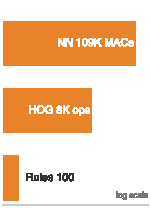
\includegraphics[height=4.4cm]{images/modules/TH-9/vol1_nn_computation_margin_001.pdf}
    \end{column}
    \begin{column}{0.54\textwidth}
      \small
      \begin{itemize}
        \item The written rules of the running example need about 100
              comparisons.
        \item The learned features need about 8 000 operations.
        \item The neural network needs 109 184 multiply-accumulate
              operations.
      \end{itemize}
    \end{column}
  \end{columns}
  \vskip 0.3em
  \small The change is not free. A model buys its rules with arithmetic.
  \source{Figure adopted from Volume I, chapter 5, and the operation counts
    of its running example.}
\end{frame}

% ----------------------------------------------- 20. the step in the middle
\begin{frame}{There is a step between the two paradigms}
  \begingroup\centering
  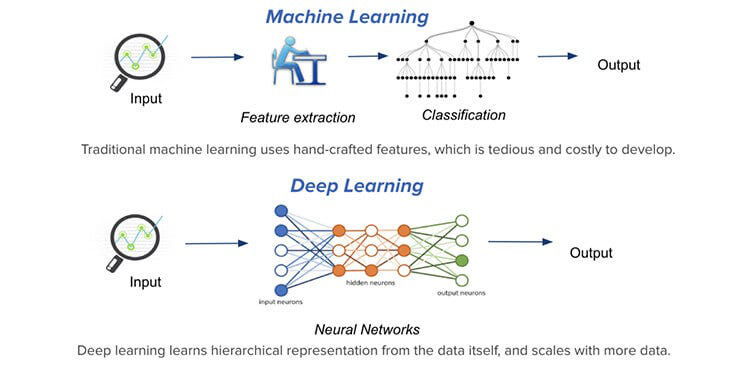
\includegraphics[width=0.78\textwidth]{images/modules/TH-9/ml_vs_deep_learning.png}
  \par\endgroup
  \vskip 0.4em
  \small The upper row asks a person to design the features. The lower row
  lets the training design them. The middle option is the most common today
  on a small device.
  \source{Figure adopted from Volume I, chapter 5.}
\end{frame}

% ----------------------------------------------------------- 21. the decision
\begin{frame}{Which tool does the problem need}
  \footnotesize
  \begin{tabular}{@{}L{4.3cm}L{4.6cm}@{}}
    \toprule
    Use written rules when & Use a learned model when \\
    \midrule
    The states can be listed & The states cannot be listed \\
    The right answer is exact & The right answer is close enough \\
    A wrong answer shows at once & A wrong answer stays hidden \\
    The rules change often & The rules change with the data \\
    \bottomrule
  \end{tabular}
  \vskip 0.5em
  \small Most systems hold both. A thermostat reads a number with a written
  rule and decides "this person fell" with a model.
  \vskip 0.3em
  \keypoint{Ask what the wrong answer costs. That question has no rule.}
\end{frame}

% -------------------------------------------------------------- 22. fallacies
\begin{frame}{Three mistakes}
  \small
  \begin{itemize}
    \item \textbf{A model replaces the program.} It replaces the rules
          inside the program. The sensor, the timing, and the memory budget
          stay.
    \item \textbf{More data removes the work.} More data removes the rule
          count. It does not remove the labels, the hardware, or the test
          on unseen data.
    \item \textbf{A learned model is always the smaller program.} The model
          of the running example needs about 1 100 times the arithmetic of
          the written rules, so the budget moves to the arithmetic.
  \end{itemize}
  \vskip 0.4em
  \keypoint{Learning moves the difficulty. It does not remove it.}
\end{frame}

% --------------------------------------------------------------- 23. summary
\begin{frame}{What to remember}
  \small
  \begin{enumerate}
    \item Written rules and a learned model give an answer. The difference
          is where the rules live.
    \item Four parts: features, labels, model, and loss.
    \item The training is a loop of predict, measure, and move. The
          inference is the forward pass alone.
    \item Regression answers with a number. Classification answers with a
          class.
    \item The decision rests on what a wrong answer costs.
  \end{enumerate}
\end{frame}

% --------------------------------------------------------------- exercise
\exerciseframe{Rules or model}{A team has three problems.
\begin{enumerate}
  \item A smart lock must open when the six digits of a code match the six
        digits that are stored.
  \item A watch must count the steps of a person from the readings of its
        accelerometer.
  \item A camera must find the three defects on the printed circuit boards
        that leave the factory.
\end{enumerate}

For each problem, decide if written rules or a learned model is the correct
tool, and give one reason.
}

\answerframe{Rules or model}{
  \begin{enumerate}
    \item \textbf{Written rules.} The correct answer is exact, and a wrong
          answer is visible at once: the lock does not open. The states
          can be listed, because a code is six digits.
    \item \textbf{A learned model.} The correct pattern of the readings is
          not known in advance, and it changes with the person and with the
          position of the watch. A wrong step count stays hidden, so the
          cost of the mistake is low and the number of cases is large.
    \item \textbf{A learned model.} The position and the light of the
          defects vary, and nobody can list them. A wrong answer on a board
          that is good is the normal case, so the model must be measured on
          real boards.
  \end{enumerate}
  \vskip 0.3em
  \small The rule that separates the three cases is the cost of the wrong
  answer. A lock that stays shut costs little, so a simple rule is enough.
  A board that ships with a defect costs a customer, so the tool must find
  the rare case.
}